\section{Projektmanagement}
Für das gemeinsame Verständnis des Begriffes ``Projektmanagement'' wird zuerst
eine Definition des Wortes gemacht. Danach wird näher auf den Aufbau eines
Projektablaufes eingegangen.

\subsection{Begriffserklärung}
Im Rahmen eines Projektmanagement werden die diversen Aufgaben ganzheitlich in
einem Projekt eingebettet und unter Berücksichtigung der Parameter Kosten, Termine
und Qualität geplant und durchgeführt.\footnote{\citealp*[Vgl.][S. 9]{burghardt2007einfuehrung}}
Die Stiftung für Forschung und Beratung am Betriebswissenschaftlichen Institut 
(BWI) der ETH Zürich definiert den Begriff Projektmanagement wie folgt:

\begin{quote}
``Projektmanagement wird als Überbegriff aller planenden, überwachenden,
koordinierenden und steuernden Massnahmen verstanden, die für die Um- oder
Neugestaltung von Systemen (resp. Problemlösungen) erforderlich sind.''\footnote{\citealp*[S. 1.1]{stiftung1998projekt}}
\end{quote}

\subsection{Projektablauf}
Der Projektablauf gehört zu den Methoden und Techniken der Organisation. Als
Projekt bezeichnet man ein Vorhaben, das einmalig ist und einen definierten
Start- und Endtermin hat. Im Projektablauf regelt man die Ablauforganisation
eines Projektes, also welche Aufgaben wann zu erledigen sind.\footnote{\citealp*[Vgl.][S. 136]{schmidt2002einfuehrung}}
Das Projektmanagement mit dem Projektablauf als Methode umfasst alle Aktivitäten,
die für eine vollständige Abwicklung eines Projektes erforderlich sind.\footnote{\citealp*[Vgl.][S. 11]{burghardt2007einfuehrung}}

Ein Projektablauf unterteilt man in vier Hauptabschnitte, die in der Abbildung \ref{pic:01_hauptabschnitte}
dargestellten sind.

\begin{figure}[htbp]
\begin{center}

\includegraphics[width=0.85\textwidth,angle=0]{./bilder/theorie/01_hauptabschnitte.pdf}
\caption{Vier Hauptabschnitte eines Projektablaufes}
\label{pic:01_hauptabschnitte}
\end{center}
\end{figure}

\subsubsection{Projektdefinition}
Die Projektdefinition besteht aus der eigentlichen Gründung eines Projektes,
der Definition des Projektziels und die Organisation des Projektes.

Zu Beginn eines Projektes steht der Projektantrag. Er beinhaltetet alle relevanten
Informationen wie eine Aufgabenbeschreibung und Termine. Wird der Projektantrag
angenommen, wandelt sich der Antrag in einen Projektauftrag um.\footnote{\citealp*[Vgl.][S. 13]{burghardt2007einfuehrung}}
Als nächstes muss ein eindeutiges und vollständiges Projektziel definiert werden.
Dies geschieht meist zusammen mit dem Auftraggeber anhand eines Anforderungskatalogs
oder Pflichtenhefts.

Es empfiehlt sich eine Problemfeldanalyse und eine Wirtschaftlichkeitsbetrachtung
zu machen. Ohne genauere Kenntnisse zur Wirtschaftlichkeit eines Projektes sollte
keines begonnen werden.\footnote{\citealp*[Vgl.][S. 45]{burghardt2007einfuehrung}}
Danach müssen die organisatorischen Voraussetzungen für das Projekt geschaffen werden,
indem der Projektleiter ernannt und eine passende Projektorganisation gewählt wird.
Die Definition einer Projektorganisation lautet nach DIN 69901:

\begin{quote}
Gesamtheit der Organisationseinheiten und der aufbau- und ablauforganisatorischen
Regelungen zur Abwicklung eines bestimmten Projektes.
\end{quote}

\subsubsection{Projektplanung}
In der Projektplanung definiert man die Strukturplanung, eine Aufwandschätzung,
die Arbeits- und Kostenplanung sowie das Risikomanagement.

In der Strukturplanung wird das Vorhaben technisch, aufgabengemäss und kaufmännisch
anhand den Anforderungen strukturiert. Auf den sich ergebenden Strukturen bauen
alle weiteren Planungsschritte auf. Danach werden daraus die einzelnen Aufgabenpakete
abgeleitet, für die dann eine Aufwandsschätzung durchzuführen ist.\footnote{\citealp*[Vgl.][S. 14]{burghardt2007einfuehrung}}
Wenn möglich sollten zur Schätzung nebst dem eigenen Erfahrungspotential auch
Erfahrungen von Experten zum Thema herangezogen werden.

Ein allgemeines Schema\footnote{Eigene Darstellung des Schemas in Anlehnung an \citealp*[S. 112]{litke2007projektmanagement}}
zur Vorgehensweise zum Sammeln von Erfahrungswerten zur Aufwandsschätzung ist in der Grafik \ref{pic:02_schema_aufwandsschaetzung}
abgebildet.

\begin{figure}[htbp]
\begin{center}
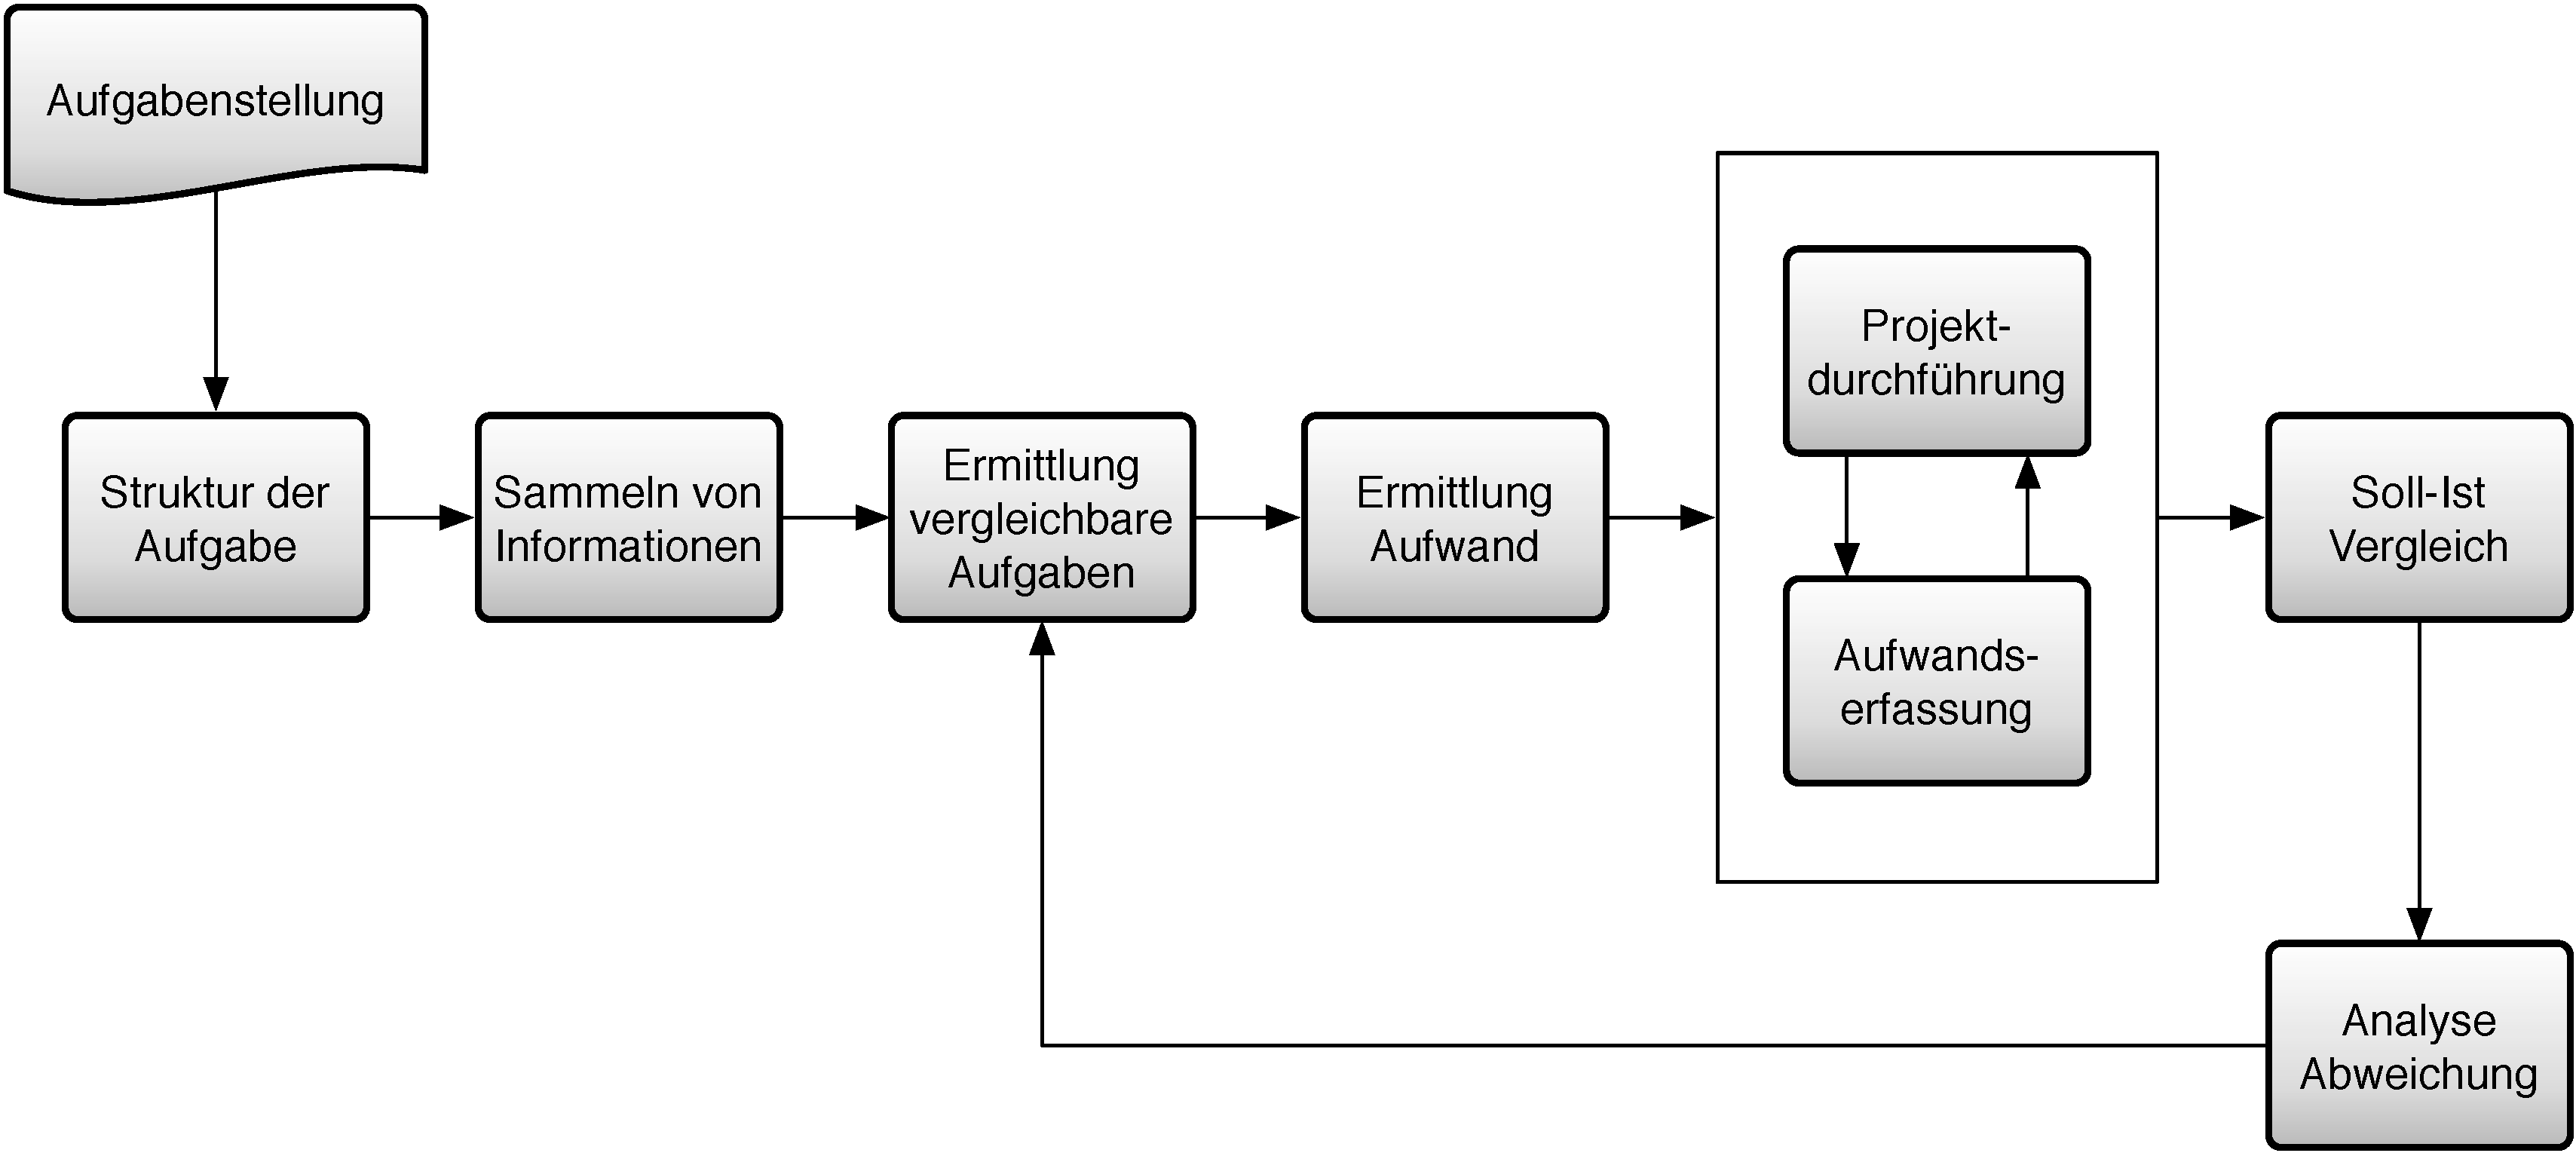
\includegraphics[width=0.95\textwidth,angle=0]{./bilder/theorie/02_schema_aufwandsschaetzung.pdf}
\caption{Sammeln von Erfahrungswerten zur Aufwandsschätzung}
\label{pic:02_schema_aufwandsschaetzung}
\end{center}
\end{figure}

Es gibt diverse Aufwandsschätzungsverfahren die genutzt werden können. Die Methoden unterscheiden
sich beim Schätzverfahren\footnote{Vgl. \citealp*{noth1986aufwandschaetzung} und \citealp*{knoell1991aufwandsschaetzung}}
und können zum Beispiel nach folgender Klassifikation erfolgen:

\begin{itemize}
    \item Anzahl der Phasen, die abgedeckt werden, zum Beispiel:
    \begin{itemize}
        \item Einzelaktivitäten
        \item Programmierung
        \item Detailentwurf und Programmierung
        \item Gesamter Entwicklungsprozess
    \end{itemize}
    \item Theoretische oder praktische Absicherung, zum Beispiel:
    \begin{itemize}
        \item Unternehmensspezifische Verfahren
        \item Unternehmensunabhängige Praxisverfahren
        \item Wissenschaftlich fundierte Verfahren
    \end{itemize}
    \item Verwendungszweck, zum Beispiel:
    \begin{itemize}
        \item Kosten/Nutzenanalyse zur Kalkulation der Kosten
        \item Kapazitäts- und Terminplanung zur Ermittlung von Plangrössen
    \end{itemize}
\end{itemize}

Anhand den Ergebnissen aus der Aufwandsschätzung werden nun die einzelnen
Arbeitspakete bzw. Teilaufgaben in eine Arbeitsplanung übernommen. Oft empfiehlt
es sich hier einen Netzplan zur Erstellung der Aufgaben- und Terminplanung
anzufertigen. ``Die Netzplantechnik ist trotz aller Kritik eines der 
leistungsfähigsten Projektmanagement-Hilfsmittel, wenn sie richtig eingesetzt wird.''
\footnote{\citealp*[S. 14]{burghardt2007einfuehrung}}

\begin{figure}[htbp]
\begin{center}
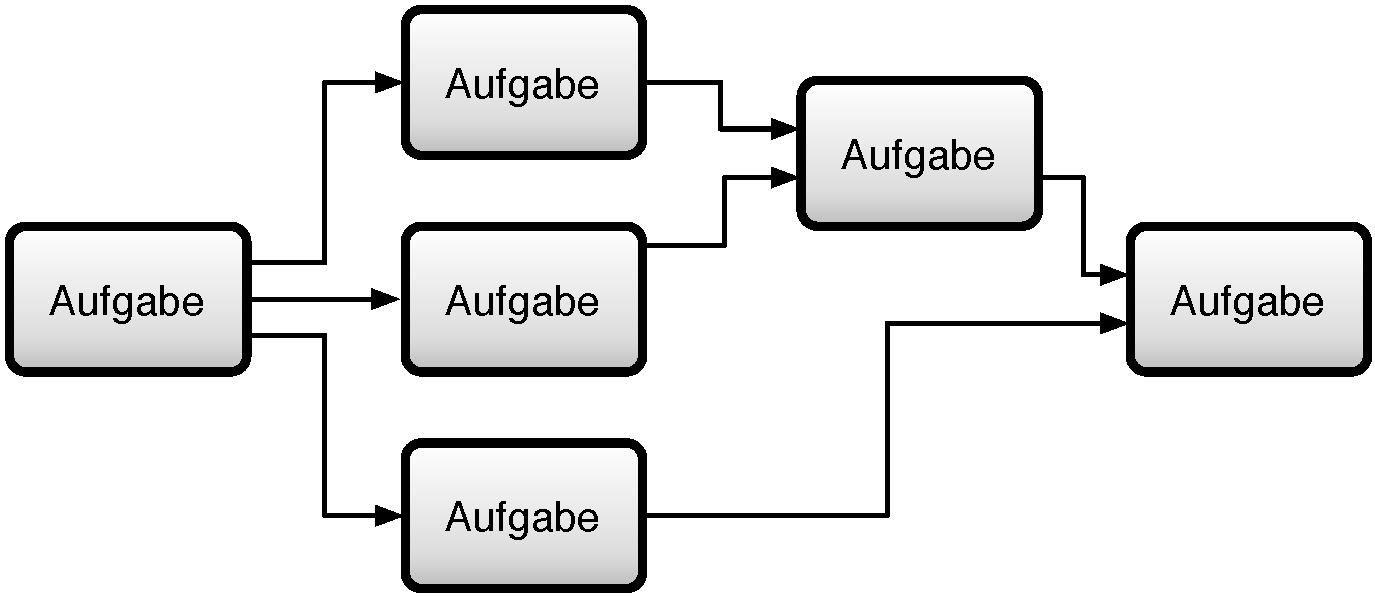
\includegraphics[width=0.5\textwidth,angle=0]{./bilder/theorie/03_darstellung_netzplan.pdf}
\caption{Konzeptionelle Darstellung eines determinisitischen Netzplanes}
\label{pic:03_darstellung_netzplan}
\end{center}
\end{figure}

% http://books.google.de/books?id=m54LKbnCIoYC&pg=PA155&dq=Netzplantechnik&hl=de&ei=Qai-Tf2dNsmDOqL12dsF&sa=X&oi=book_result&ct=result&resnum=9&ved=0CHYQ6AEwCA#v=onepage&q=Netzplantechnik&f=false

\subsubsection{Projektkontrolle}
An erster Stelle der Projektkontrolle steht der Plan/Ist-Vergleich der vorgegebenen
Projektparameter. Durch einen laufenden Vergleich im Rahmen der Projektkontrolle
erreicht man, dass Abweichungen frühzeitig erkannt werden. Diese Abweichungen
führen zu ``geeigneten'' Massnahmen, die rechtzeitig ergriffen werden können.
Die Projektkontrolle umfasst im ganzen die Termin-, Aufwands-, Kosten-, 
und Sachfortschrittskontrolle, Qualitätssicherung, Projektdokumentation und
das Personalmanagement.\footnote{\citealp*[Vgl.][S. 15]{burghardt2007einfuehrung}}

Die Terminkontrolle wird in der Praxis so umgesetzt, dass die Einhaltung
und Erreichung der gesetzten Meilensteine kontrolliert wird. Wenn ein 
Meilenstein nicht eingehalten werden kann, muss kontrolliert werden, ob die
weiteren davon betroffen sind. Häufig ist das der Fall und die Termine
müssen angepasst und neu gewählt werden. Hierbei ist es wichtig, den Auftraggeber
über die Veränderungen zu informieren.

Die Aufwands- und Kostenkontrolle wird in der Praxis meist durch die Kontrolle
der rapportierten Stunden durchgeführt. Man sollte in beiden Fällen, also der
Termin- und Aufwandskontrolle, eine Trendanalyse erstellen, um eine mögliche
Entwicklung daraus abzuleiten.

Die Sachfortschrittskontrolle ist eine der wichtigsten Kontrollaufgaben für
den Projektleiter. Es ist zuggleich aber auch die schwierigste, da oft keine
unmittelbare Messgrössen vorhanden sind. ``Grundsätzlich ist es empfehlenswert,
während der Projektdurchführung in bestimmten Abständen Restaufwands- und
Restzeitschätzungen vorzunehmen.''\footnote{\citealp*[S. 16]{burghardt2007einfuehrung}}

Bei der Projektdokumentation handelt es sich um die vollständigen Informationen
über das zu entwickelnde Produkt. Es empfiehlt sich eine Projektakte mit einer
vorgegebenen Ordnung aufzubauen und eine Art Projekttagebuch zu führen, dessen
Inhalt an keine Ordnungssystematik gebunden ist. Die daraus abzulesenden
Informationen werden zur Projektberichterstattung verwendet.

Das Personalmanagement in einem Projekt beinhaltet eine projektkonforme
Personalführung und das Fördern einer positiven Zusammenarbeit in einem
Projektteam. Wichtig ist stets die Akzeptanz der Projektleitung und die 
Motivation der Projektmitarbeiter. Ein gutes Konfliktmanagement spielt
dabei ebenfalls eine wichtige Rolle, damit man auf Konflikte innerhalb des
Projektes frühzeitig reagieren und sie bewältigen kann. Projektmanagement
wird oft auch als ``permanentes Konfliktmanagement'' bezeichnet. Dabei ist es
wichtig, dass Konflikte als etwas Normales und als Aufgaben oder zu lösende 
Probleme angesehen werden.\footnote{\citealp*[S. 119]{kessler2004projektmanagement}}

\subsubsection{Projektabschluss}
Der Projektabschluss umfasst die Schritte Produktabnahme, Projektabschluss,
Erfahrungssicherung und Projektauflösung.

Der Projektabschluss wird durch die Produktabnahme eingeleitet. Im besten Fall
wird der Abnahmetest durch eine entwicklungsunabhängige Stelle durchgeführt.
Die Übergabe an den Auftraggeber ist in einem Produktabnahmebericht festzuhalten.
Der Produktabnahmebericht sollte eine Beschreibung der Ergebnisse und eventuelle
Nachforderungen beinhalten. In der Regel beginnt nach der Abnahme die
Gewährleistungsfrist. Das bedeutet, dass der Zeitpunkt der Produktabnahme von
rechtlicher Relevanz sein kann und der Produktabnahmebericht vom Auftraggeber
unterschrieben werden sollte.\footnote{\citealp*[Vgl.][S. 86]{cronenbroeck2004handbuch}}
Zu diesem Zeitpunkt sollte man sich auch Gedanken über eine zukünftige Betreuung
machen.

In der Projektabschlussanalyse wird die ehemals erstellte Wirtschaftlichkeitsrechnung
auf ihre Einhaltung durchleuchtet. Zusätzlich werden die Einhaltung der Termine sowie
Leistungs- und Qualitätsmerkmale betrachtet. Wichtige Kennzahlen sind zudem
die Änderungshäufigkeit und Fehlerquote.\footnote{\citealp*[Vgl.][S. 265]{schelle2007projekte}}
Grundsätzlich sollten alle gesammelten Daten in eine Art Erfahrungsdatenbank 
des Unternehmens einfliessen. Diese stellen eine wichtige Voraussetzung für das 
Optimieren von Aufwandsschätzungen dar und können somit auf zukünftige Projekte 
eine positive Wirkung haben.\footnote{\citealp*[Vgl.][S. 275]{burghardt2007einfuehrung}}

\begin{figure}[htbp]
\begin{center}
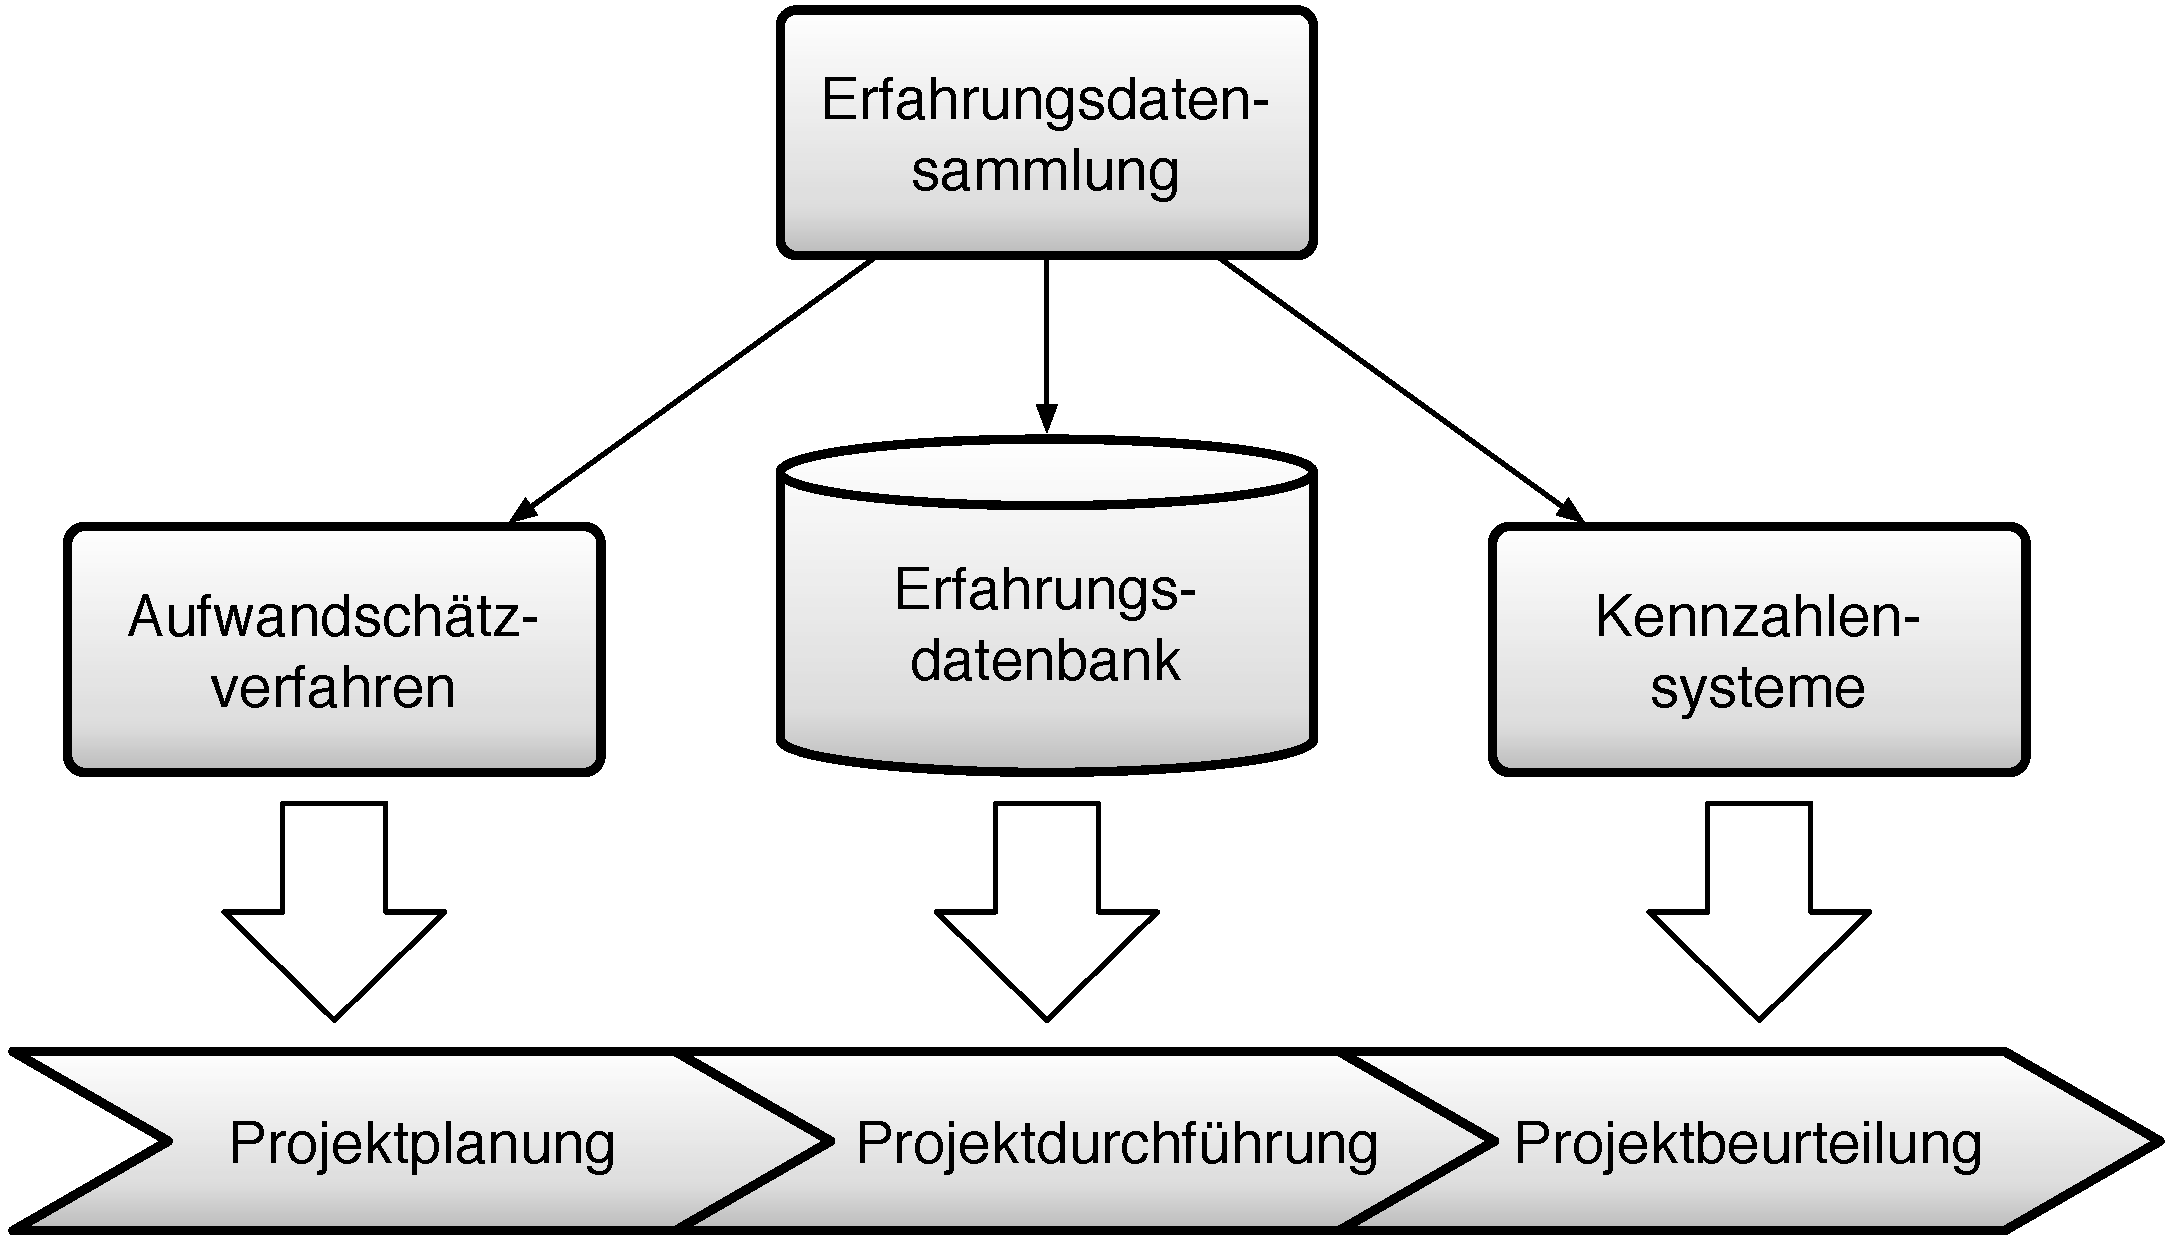
\includegraphics[width=0.6\textwidth,angle=0]{./bilder/theorie/04_unterteilung_erfahrungsdaten.pdf}
\caption{Unterteilung der Erfahrungsdaten}
\label{pic:04_unterteilung_erfahrungsdaten}
\end{center}
\end{figure}

Die Projektauflösung ist der letzte Schritt in der Projektabschlussphase. Wie 
zu Beginn erwähnt soll jedes Projekt auch ein eindeutiges Ende haben. Dies ist
für das Projektpersonal besonders wichtig, da sie dann offiziell von dem
Projekt entbunden sind und in neue Projekte und Aufgaben übergeleitet werden
können. Möglicherweise ist es je nach Projekt auch sinnvoll, einen Abschluss
gebührend zu feiern.